\chapter{Implementation and Assessment}
\label{chp:Implementation_and_Assessment}

All algorithms discussed in this work are realized in \mbox{MATLAB}, a 

\section{Requirements}

For the implementation and physical realization, some 

\section{Oversampling}

\section{Baseline Scaling and Back Projection}

\section{Attenuator Tiling and Blending}

High resolution light fields can take up a significant amount of space in memory. 
For example, a light field taken with a Full HD camera from $17 \times 17$ angles would take up $1920 \cdot 1080 \cdot 17^2 \cdot 3 \cdot 8 / (1024^3) = 13.3947$ Gigabyte of memory. 
In addition, the propagation matrix stores information about every pixel in the light field and thus, can take up Gigabytes of space depending on the resolution of the attenuation layers. 
The proposed approach divides the attenuation layers into tiles. 
Figure~\ref{fig:tiling_layout} shows how the tiles are laid out.
\begin{figure}[tb]
	\begin{subfigure}{0.5\textwidth}
		\centering
		\documentclass{standalone}
\usepackage{tikz}

\begin{document}
	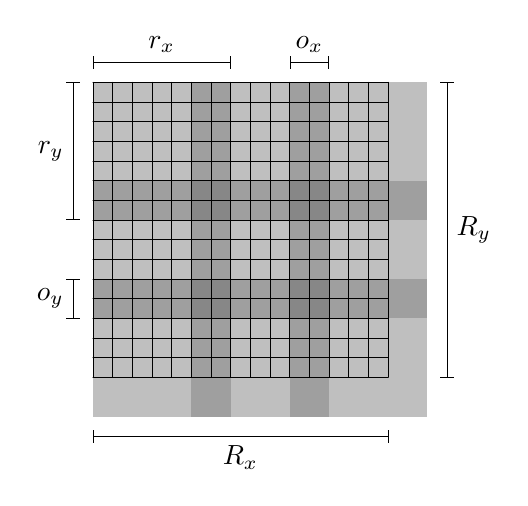
\begin{tikzpicture}[scale = 0.25, very thin]
	
		% Tiles
		\foreach \x in {0,...,2} {
			\foreach \y in {0,...,2}{
				\fill[gray, opacity = 0.5] (\x * 5, -\y * 5) rectangle ++(7, -7);
			}
		}
		
		% Grid
		\draw[step = 1 cm, cap = round] (0, 0) grid (15, -15);
		
		% Markers
		\draw[|-|] (0, -18) -- node[below]	{$R_x$} ++(15, 0);
		\draw[|-|] (18, 0) -- node[right]	{$R_y$} ++(0, -15);
		\draw[|-|] (0, 1) 	-- node[above]	{$r_x$} ++(7, 0);
		\draw[|-|] (-1, 0) 	-- node[left]	{$r_y$} ++(0, -7);
		\draw[|-|] (10, 1) 	-- node[above]	{$o_x$} ++(2, 0);
		\draw[|-|] (-1, -10) -- node[left]	{$o_y$} ++(0, -2);
	
	\end{tikzpicture}
\end{document}

		\caption{}
		\label{fig:tiling_layout}
	\end{subfigure}%
	\begin{subfigure}{0.5\textwidth}
		\centering
		\documentclass{standalone}
\usepackage{calc}
\usepackage{tikz}

\begin{document}
	\begin{tikzpicture}[scale = 0.25, very thin]
	
		% Tiles
%		\foreach \x in {0,...,2} {
%			\foreach \y in {0,...,2}{
%				\fill[gray, opacity = 0.5] (\x * 5, -\y * 5) rectangle ++(7, -7);
%			}
%		}

		% Summed up masks
		\node [anchor = north west, inner sep = 0] at (0, 0) {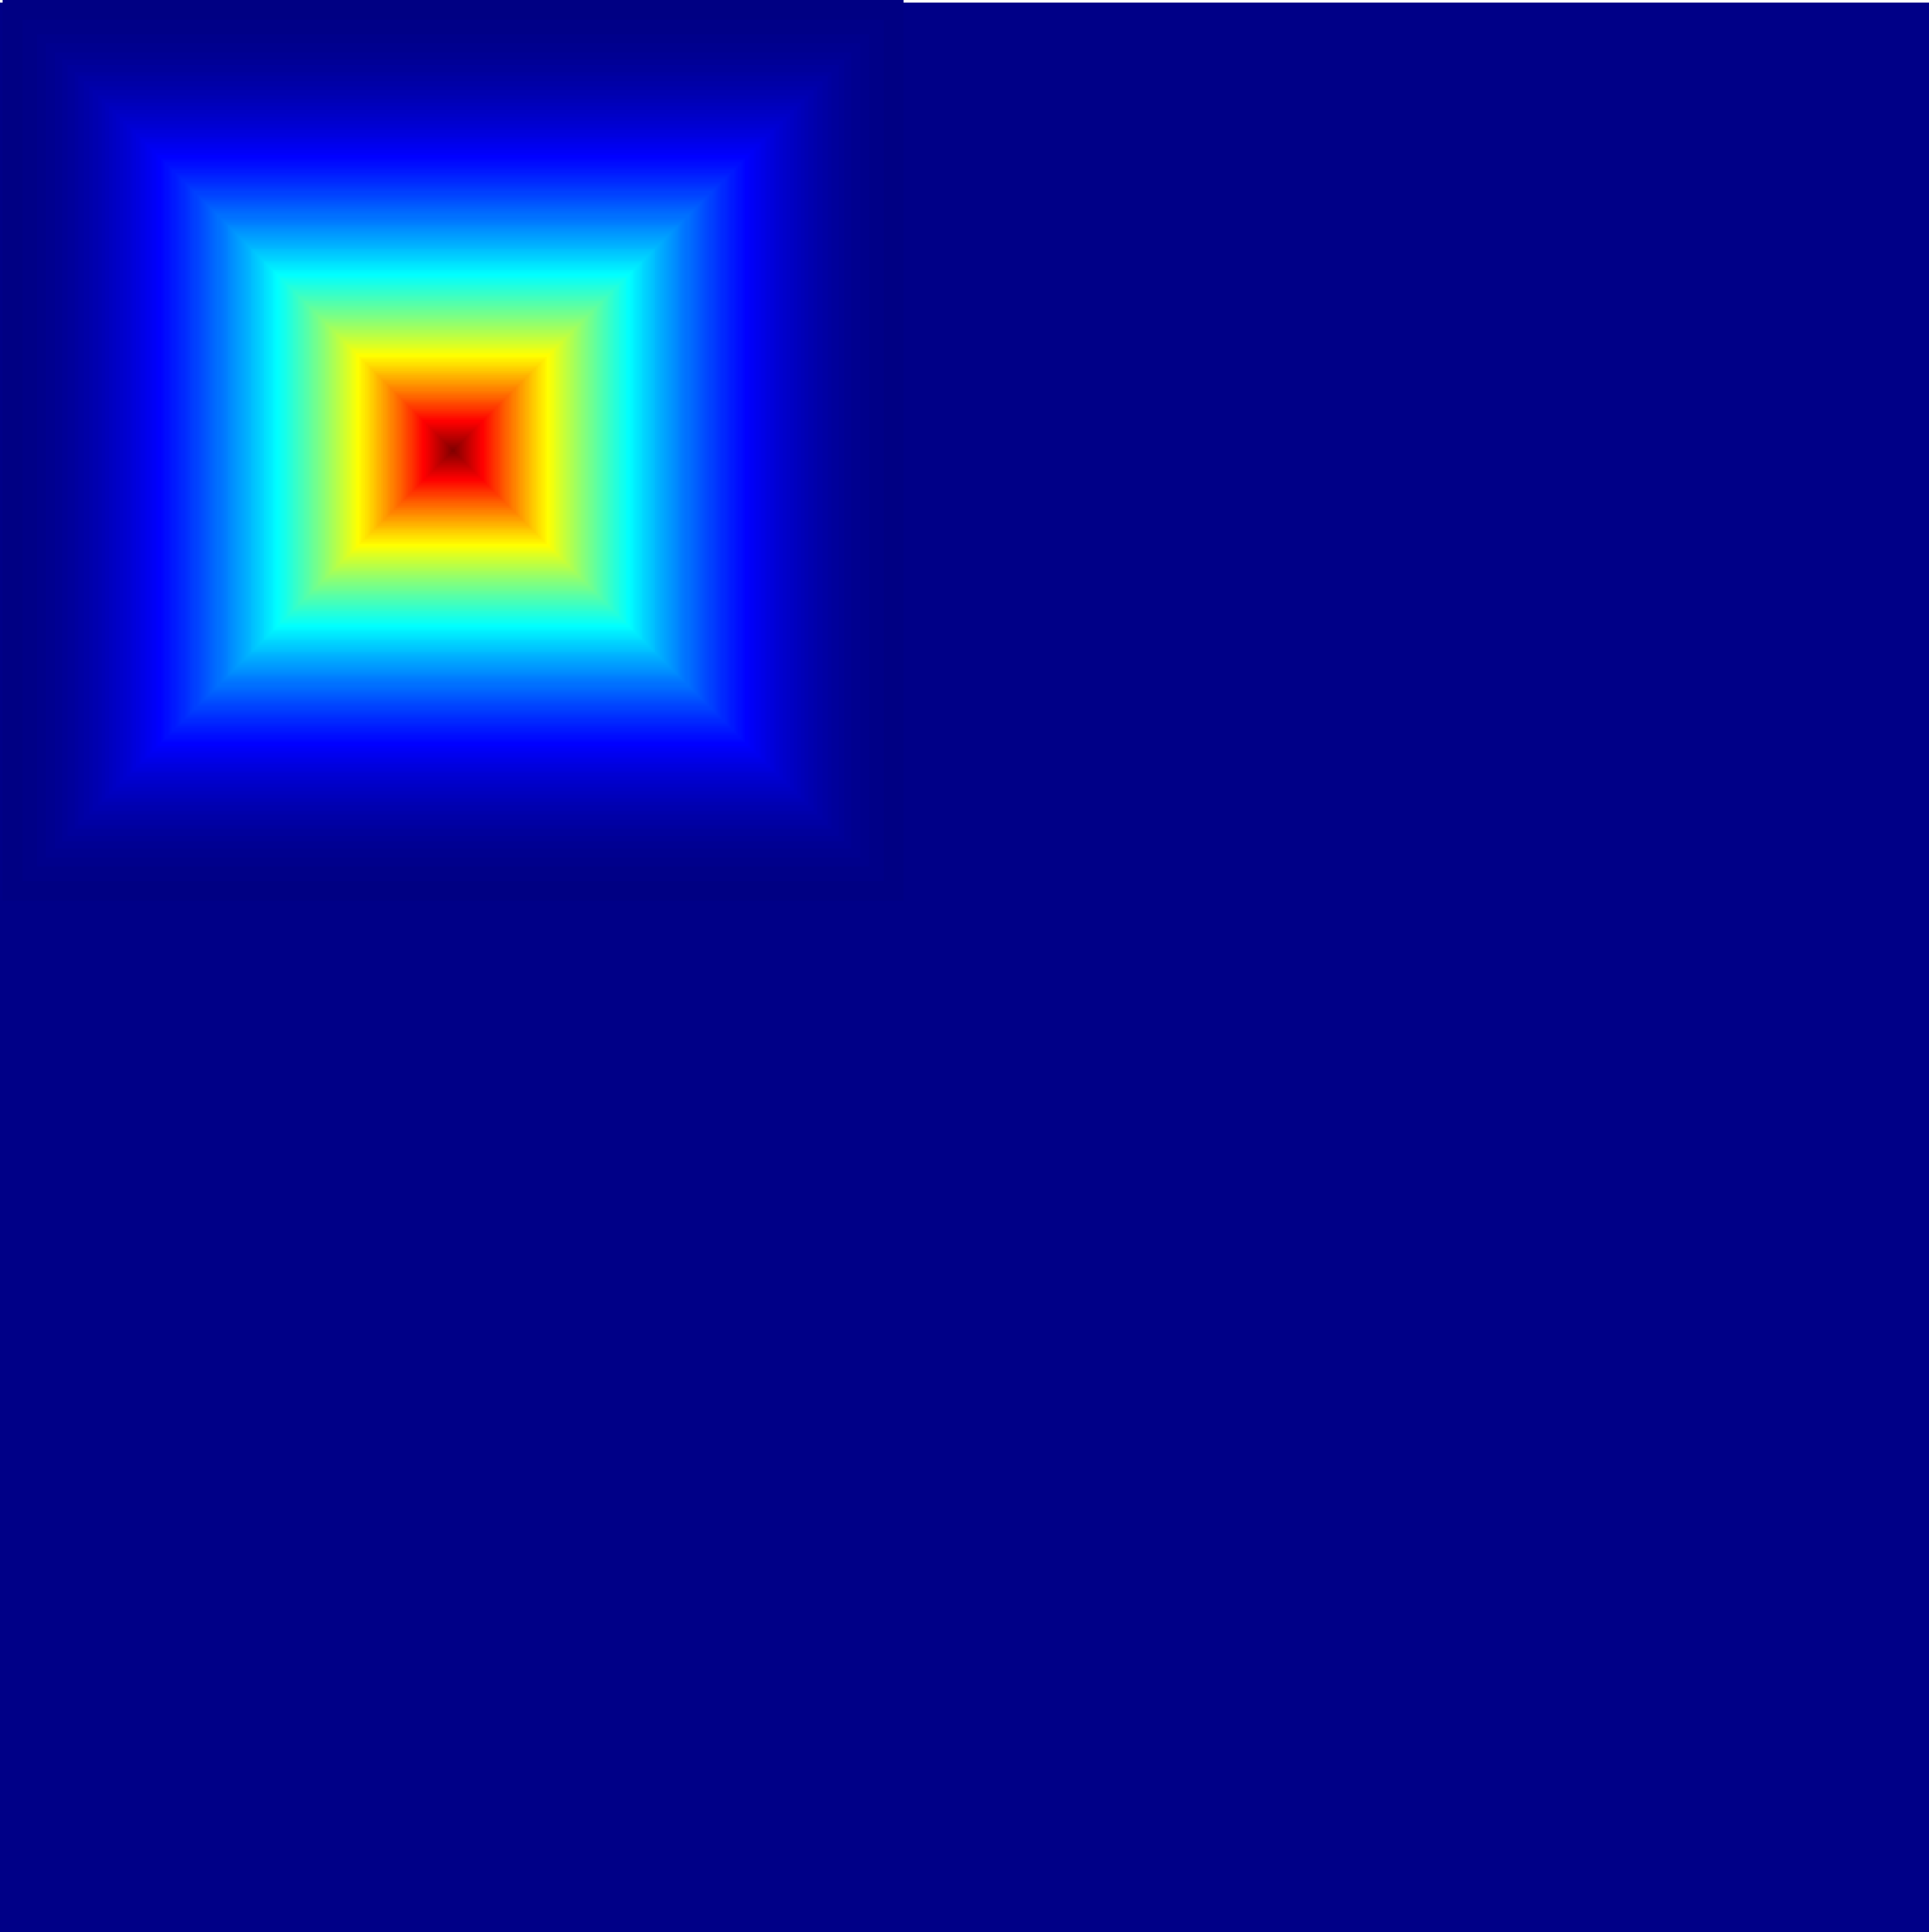
\includegraphics[width = 3.75cm]{./figures/tiling/mask1}};
		\node [anchor = east, scale=2] at (-0.5, -3.6) {$\ast$};
		% Grid
%		\draw[step = 1 cm, cap = round] (0, 0) grid (15, -15);
		
		% Invisible markers for accurate placement in figure 
		\begin{scope}[opacity = 0]
			\draw[|-|] (0, -18) -- node[below]	{$R_x$} ++(15, 0);
%			\draw[|-|] (18, 0) -- node[right]	{$R_y$} ++(0, -15);
			\draw[|-|] (0, 1) 	-- node[above]	{$r_x$} ++(7, 0);
%			\draw[|-|] (-1, 0) 	-- node[left]	{$r_y$} ++(0, -7);
			\draw[|-|] (10, 1) 	-- node[above]	{$o_x$} ++(2, 0);
%			\draw[|-|] (-1, -10) -- node[left]	{$o_y$} ++(0, -2);
		\end{scope}
		
	\end{tikzpicture}
\end{document}
		\caption{}
		\label{fig:sum_of_quadratic_blending_masks}
	\end{subfigure}%
	\caption[Tiling layout]
			{(a) Layout of the tiles that cover the attenuation layers.
				 The pixel grid of size $R_x \times R_y$ is covered by tiles of $r_x \times r_y$ pixels with an overlap of $o_x$ in horizontal and $o_y$ in vertical direction.
			 (b) The sum of the per-tile quadratic blending masks used for the normalization.}
\end{figure} 
The inputs for the tiling algorithm are the resolution of the tiles $r = (r_x, r_y)$ and the overlap in horizontal and vertical direction, $o = (o_x, o_y)$. 
The tiles are then laid out in a grid beginning in the top left corner of the layer. 
The number of tiles needed to cover the plane can be calculated by 
\begin{equation}
	N_x = \left \lceil \dfrac{R_x - o_x}{r_x - o_x} \right \rceil
	\qquad 
	\text{and} 
	\qquad
	N_y = \left \lceil \dfrac{R_y - o_y}{r_y - o_y} \right \rceil.
\end{equation}
The combination of the same tile from each layer forms a new attenuator of smaller size and lower resolution. 
The optimization is then performed for every tile separately, resulting in a smaller propagation matrix per tile. 
In the end, the optimized tiles are put together to form the complete attenuation layers. 

In general, the borders of the attenuator contain less ray-propagation information and thus provide a higher degree of freedom for the optimization. 
This introduces artifacts that are clearly visible in the reassembled layers as shown in figure~\ref{fig:comparison_tile_overlap_vs_no_overlap}.
\begin{figure}[tb]
	\centering
	\begin{subfigure}{0.23\textwidth}
		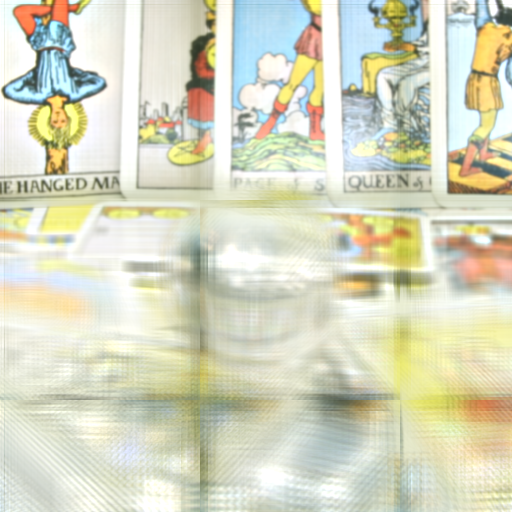
\includegraphics[width = \textwidth]{../Figures/tiling/tarot_tiles3x3x200x200_no_overlap_3_layers/1.png}
		
		\vspace{0.15cm}
		
		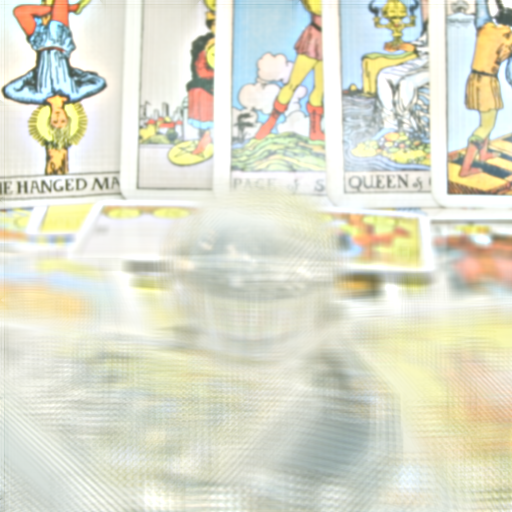
\includegraphics[width = \textwidth]{../Figures/tiling/tarot_tiles5x5x200x200_overlap0.5_3_layers/1.png}
		\caption{Layer 1}
	\end{subfigure}\hspace{0.15cm}%
	\begin{subfigure}{0.23\textwidth}
		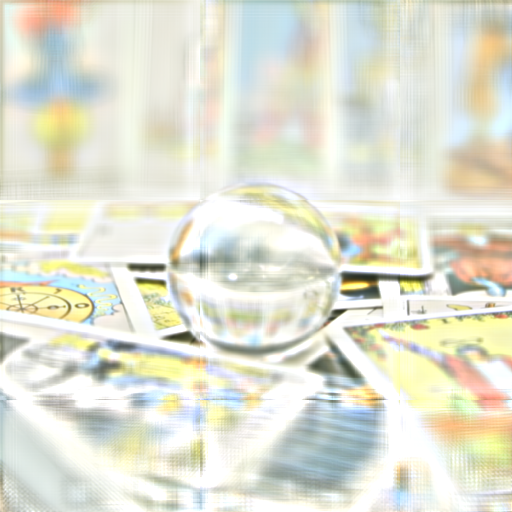
\includegraphics[width = \textwidth]{../Figures/tiling/tarot_tiles3x3x200x200_no_overlap_3_layers/2.png}
		
		\vspace{0.15cm}
		
		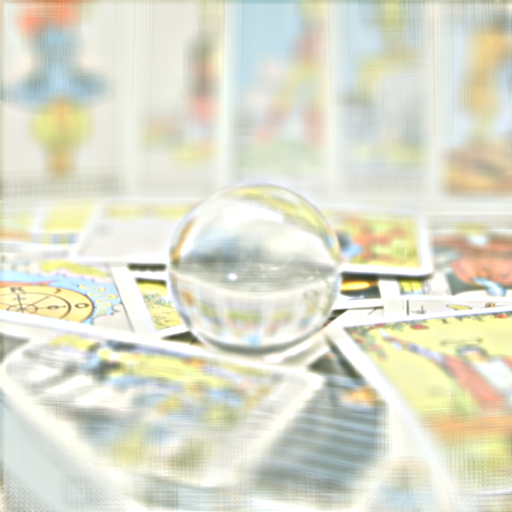
\includegraphics[width = \textwidth]{../Figures/tiling/tarot_tiles5x5x200x200_overlap0.5_3_layers/2.png}
		\caption{Layer 2}
	\end{subfigure}\hspace{0.15cm}%
	\begin{subfigure}{0.23\textwidth}
		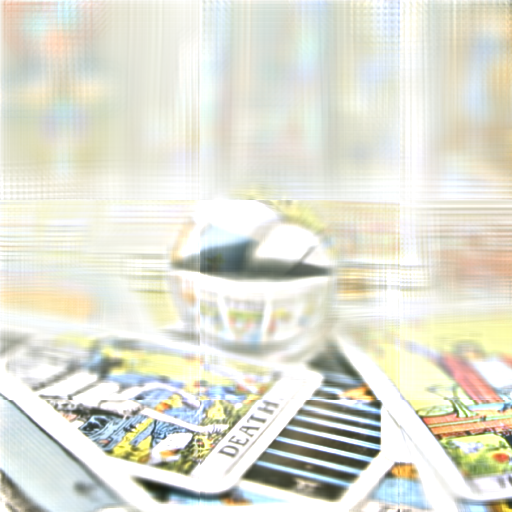
\includegraphics[width = \textwidth]{../Figures/tiling/tarot_tiles3x3x200x200_no_overlap_3_layers/3.png}
		
		\vspace{0.15cm}
		
		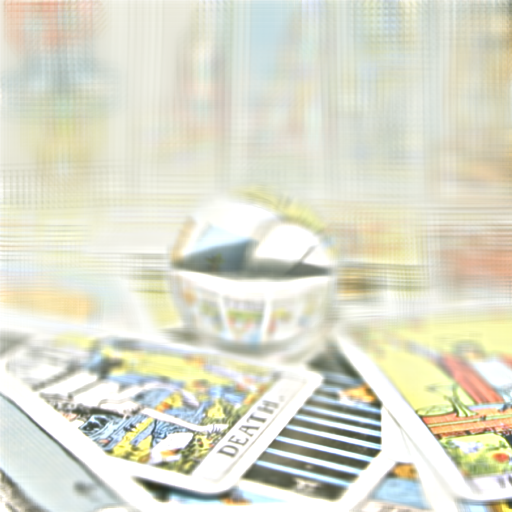
\includegraphics[width = \textwidth]{../Figures/tiling/tarot_tiles5x5x200x200_overlap0.5_3_layers/3.png}
		\caption{Layer 3}
	\end{subfigure}\hspace{0.15cm}%
	\begin{subfigure}{0.23\textwidth}
		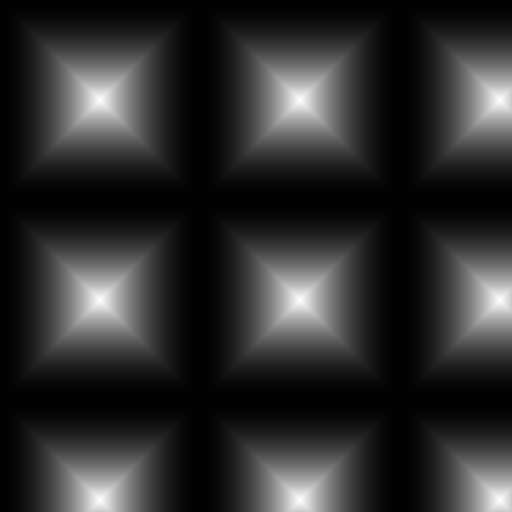
\includegraphics[width = \textwidth]{../Figures/tiling/tarot_tiles3x3x200x200_no_overlap_3_layers/blendingMaskSum.png}
		
		\vspace{0.15cm}
		
		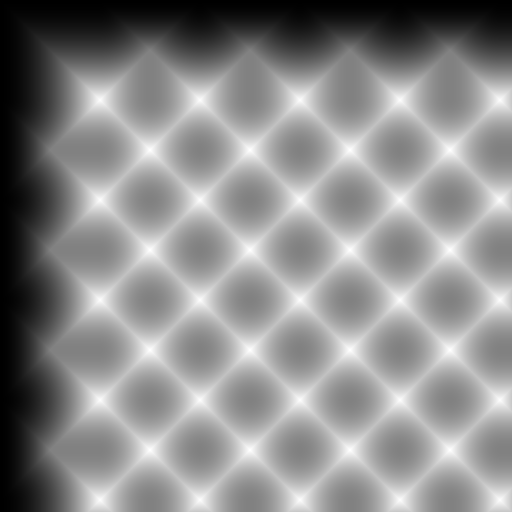
\includegraphics[width = \textwidth]{../Figures/tiling/tarot_tiles5x5x200x200_overlap0.5_3_layers/blendingMaskSum.png}
		\caption{Blending masks}
	\end{subfigure}%
	\caption[Impact of tile overlap on attenuation layers]
			{Impact of tile overlap on attenuation layers.
			 Top: Tiles have no overlap and grid artifacts are visible.
			 Bottom: With a 50\% overlap, the artifacts are no longer noticeable, but more tiles are needed.}
	\label{fig:comparison_tile_overlap_vs_no_overlap}
\end{figure} 
To solve this issue, the tiles have to overlap. 
In this case, when reassembling the layers from the tiles, the overlaps need to be blended with a mask:
After the optimization, each tile gets multiplied with a quadratic blending mask.
The finished layers are then obtained by summing the tiles and dividing by the sum of the blending masks shown in figure~\ref{fig:sum_of_quadratic_blending_masks}.

\todo{choice of quadratic masks?}

\section{Benefits and Limitations}

\todo{Optimization only for positive transmittance}
